\documentclass[a4paper,12pt]{article}
\usepackage[utf8]{inputenc}
\usepackage[]{graphicx}
\usepackage[]{amsmath}
\usepackage[]{mathbbol}
\usepackage[]{caption}
\usepackage[]{subcaption}
\usepackage[]{hyperref}


% Title Page
\title{Pathing Math (Draft)}
\author{Kieran Mattingly}
\date{}


\begin{document}
\maketitle

\section{Introduction}
\textbf{The FTC game} this year is a shooter game, where we have to intake wiffle balls from the field, sometimes autonomously. Our team has decided to use a differential drivetrain, like a tank. As we can only move forwards/backwards and turn, a good pathing system is necessary to handle fast, precise movement along curved trajectories. For this design, five variables are needed to represent the robot state at a given time: $x$ and $y$ position, $\theta$, the robot heading, $v$, the one-dimensional velocity along the heading, and the angular velocity $\dot \theta$. I have two control parameters, that correspond to the PWM duty cycle sent to the left and right motors.

\section{The Dynamical Model}
\textbf{First, the robot} dynamics are specified as a Partial Differential Equation (PDE). This equation, in index notation using Einstein summation convention, is
$$
\dot x^a = h^a_b(x)(A^b_cx^c+B^b_is^i(u) )
                                                                                                                            $$ where $x^a$ is the state vector, consisting of $\langle x, y, \theta, v, \dot \theta \rangle$. As explained in more detail later, $h^a_b(x)$, $A^b_c$, $B^b_i$, $s^i(u)$, and $u$, are the heading transformation, control-free state evolution, control response, control limiter, and control input (index has been suppressed for notational convenience), respectively. I computed these dynamics based off an (approximate) physical model of DC motors. Because mass and moment of inertia are approximately constant during play, the torque of the motors is directly proportional to the translational and rotational acceleration of the robot chassis. In theory, the proportionality constants could be calculated by weighing the robot, measuring it's moment of inertia, and looking up the motor torque, however in practice I find it simpler to tune this manually. Thus, by setting the torques on the wheels (or a value directly proportional to it), I can directly compute the acceleration. \\

                                                                                                                        The other key component about the robot dynamics I've modeled is back EMF. This is caused by the magnetic field inside the DC motor inducing a counter-torque, so at higher velocities the motor has a lower maximum torque. For example, see Figure 1.

\begin{figure}[ht]
\fbox {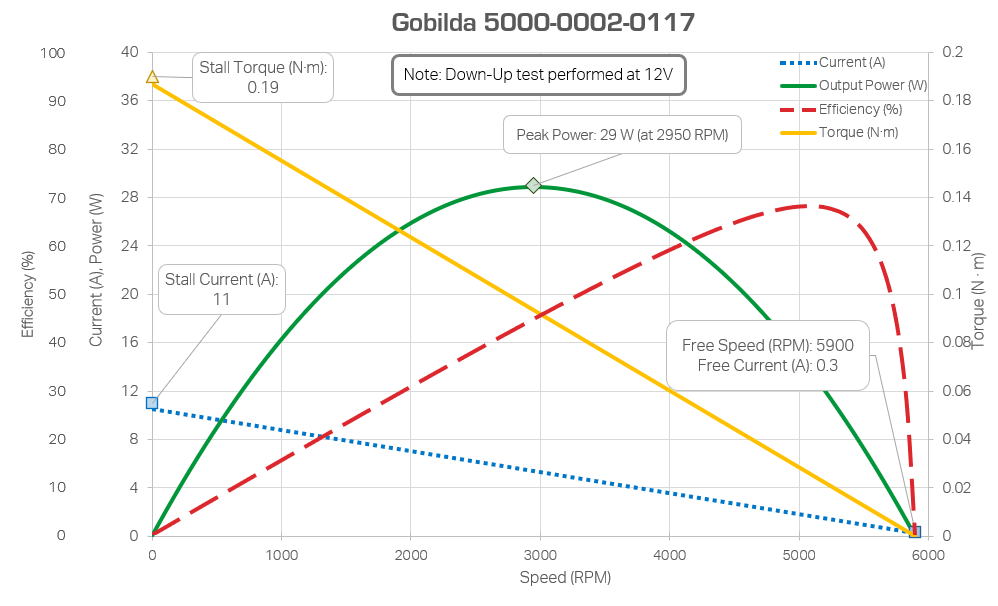
\includegraphics[width=\linewidth]{matrix-motor-curve-12V.png}}
\caption[]{A motor curve graph for one of the motors we plan on using. The yellow line represents the motor torque vs. speed. Source: Game Manual 0. (\href{https://gm0.org/ro/latest/docs/power-and-electronics/motor-guide/motor-power.html}{https://gm0.org/ro/latest/docs/power-and-electronics/motor-guide/motor-power.html})}
% matrix-motor-curve-12V.webp: 0x0 px, 300dpi, 0.00x0.00 cm, bb=
\end{figure}

Notice that it follows a decreasing linear trend. I modeled this as Stokes' drag, where the drag force is directly proportional to the velocity. However, the torque due to the control input remains constant. Thus, at high velocities, the drag force balances out the motor power, resulting in net-zero torque, and at low velocity the motor has no drag and max torque, exactly the relationship witnessed in the yellow line of the graph. Friction is handled outside this model. \\

Mathematically, this effect is in the $A$ and $B$ matrices, defined as $$
A = \begin{bmatrix}
	0 & 0 & 0 & 1 & 0\\
	0 & 0 & 0 & 0 & 0\\
	0 & 0 & 0 & 0 & 1\\
	0 & 0 & 0 & B_d & 0\\
	0 & 0 & 0 & 0 & B_\theta\\
	
	
\end{bmatrix}, \ 
B = \begin{bmatrix}
	0 & 0\\
	0 & 0\\
	0 & 0\\
	\tau_d & \tau_d \\
	-\tau_{\theta} & \tau_{\theta}\\
\end{bmatrix}
$$
Where $\tau_d$ and $\tau_\theta$ are the constant motor torques on the driving (forward) position and angle. $B_d$ and $B_\theta$ represent the negative drag coefficient on velocity in the driving direction and on the angular velocity. In the $A$ matrix is also the definition of the velocity state variables acting on position, in the first two rows. As the velocity is always in the heading direction ($\theta$), the velocity in $x$ and $y$ depends on the heading. To handle this, the $A$ matrix is defined for when $\theta = 0$, and the function $h(x)$ handles rotating the velocity to be in the direction of movement. $h(x)$ is defined to be:
$$h(x) = \begin{bmatrix}
	\cos(\theta) & -\sin(\theta) & 0 & 0 & 0\\
	\sin(\theta) & \cos(\theta) & 0 & 0 & 0\\
	0 & 0 & 1 & 0 & 0\\
	0 & 0 & 0 & 1 & 0\\
	0 & 0 & 0 & 0 & 1\\
\end{bmatrix}$$

To predict the future state, I approximated the integral of the robot dynamics equation, obtaining a state transition function $f^a(x, u) = x_{t+\Delta t}^a \approx x^a + \dot x^a \Delta t = x^a+ h^a_b(x)(A^b_cx^c + B^b_is^i(u) )\Delta t$. The $s^i(u)$ function is present to enforce control limits. I have a limit to the power I can send to the motor, so $s^i(u)$ is a sigmoid function (in this case, hyperbolic tangent) to smoothly map from $\mathbb{R} \rightarrow [-1, 1]$ (or whatever I want the control range to be). This is necessary as the control algorithm itself will assume the control input is unbounded, which results in infeasible trajectories. This concludes my dynamic model. To evaluate the accuracy, I generated a path to move forward 100 centimeters, and ran it with no feedback control. I was happy to see that, without spending too much time tuning (it was only a testing chassis), it was able to get withing 5cm of the target. In my testing, there was too much randomness (even with identical control inputs) to reliably get any closer. With feedback enabled, this shrunk to less than 3mm (Figure 2).
\begin{figure}[ht]
	\caption{Velocity vs. Time with and Without Feedback Control}
	\begin{subfigure}[t]{0.48 \textwidth}
	\includegraphics[width=\linewidth]{"No Feedback"}
	\caption{Measured (Red) vs Predicted (Blue) velocity over time without feedback control. Final positional accuracy was within 5\%. Notice that towards the end the decreased drag force causes the model to smoothly asymptote, and the data confirms this model's accuracy.}
\end{subfigure}
\hfill
\begin{subfigure}[t]{0.48 \textwidth}
	\includegraphics[width=\linewidth]{"With Correction"}
	\caption{Measured (Red) vs Predicted (Blue) velocity over time with feedback control. Notice the increased noise due to the controller correcting small errors, including errors perpendicular to the direction of motion. Final positional accuracy was within 0.3\%.}
\end{subfigure}
	
\end{figure}

\section{The Cost Function}

\textbf{Paths are} defined as a two-tuple $(X, U)$, where $X$ and $U$ are the state and control trajectories, sampled $\Delta t$ apart. In order to define what makes a trajectory "better" or "worse," however, a functional $J: X \times U \rightarrow \mathbb{R}$ must be defined. The traditional way this is done for a sequence of $n$ elements is the quadratic cost function: 
$$J(X, U) = \ell_f(x) +\sum_{k=1}^{n} \ell(x, u),$$ where
$$
\ell_f(x) = (x_n - x_{target})^TQ_f(x_n - x_{target}),$$$$
\ell(x, u) = (x_k - x_{target})^TQ(x_k - x_{target}).
$$
and $Q$ is the ongoing error cost matrix, $R$ is the control cost matrix, and $Q_f$ is the final cost matrix. This is what I currently use (although I do have ideas on how to alter this function to add obstacle avoidance and other features). Intuitively, this function makes sense; it punishes the robot for being far away from the target state for an extended period of time, but doesn't push it to the maximum control. This last part is important because it prevents the trajectory generation from resulting in a "Bang-Bang" controller, where the controls are set to their max power then minimum power. While this would be the theoretical fastest, it is not the best trajectory as it leaves no room for correction if there is an error in the model or, in this case, uncertainty. By adding in the control cost term $R$, the controller is discouraged from this behavior, helping to ensure controllability.

\section{Path Generation and Derivatives}
\textbf{The primary component} of this algorithm is the generation of paths. This is done via a technique called \textbf{Differential Dynamic Programming}, developed by Dr. Richard Bellman in the 1950s. The key idea is to, at each time step, consider what change would be the most beneficial to the path, not just at the current state, but in the future. We can recursively construct a \textit{Value} function $V$ for the current time step, by saying that $$V_k(x) = \min_u [\ell(x, u) + V_{k+1}{f(x, u)}]$$
where $f(x, u)$ is the state transition function. In effect, this means that the improvement at the current time step is how much it helps at that time step and how much it helps at the next time step. No recursion is complete without a base case, which is defined to be $V_n(x) = \ell_f(x)$, as the final cost function is itself a measure of the cost of being off at the final state. (This is a version of the \textit{Bellman equation}, restated in this particular view.)\\

To now use this equation, I initialize a nominal stationary path, and repeatedly compute an update iterativley starting from $x_n$, using Differential Dynamic Programming. Briefly stated, another function $Q$ can be defined to be the quality of an update in both state and control, taking into account robot dynamics. This can be approximated with a second-order Taylor expansion, with the following derivatives:

$$
	\begin{aligned}
		\frac {\partial Q}{\partial x^i} &= \frac{\partial \ell}{\partial x^i} + \frac{\partial f^a}{\partial x^i} \frac{\partial V}{\partial x^a} \\ 
		\frac {\partial Q}{\partial u^k} &= \frac{\partial \ell}{\partial u^k} + \frac{\partial f^a}{\partial u^k} \frac{\partial V}{\partial x^a} \\ 
		\frac {\partial^2 Q}{\partial x^i \partial x^j} &= \frac{\partial^2 \ell}{\partial x^i \partial x^j} + \frac{\partial f^a}{\partial x^i} \frac{\partial^2 V}{\partial x^a \partial x^b}\frac{\partial f^b}{\partial x^j} + \frac {\partial V}{\partial x^c} \frac{\partial f^c}{\partial x^i \partial x^j} \\ 
		\frac {\partial^2 Q}{\partial u^k \partial u^l} &= \frac{\partial^2 \ell}{\partial u^k \partial u^l} + \frac{\partial f^a}{\partial u^k} \frac{\partial^2 V}{\partial x^a \partial x^b}\frac{\partial f^b}{\partial u^l} + \frac {\partial V}{\partial x^c} \frac{\partial f^c}{\partial u^k \partial u^l}\\ 
		\frac {\partial^2 Q}{\partial u^k \partial x^j} &= \frac{\partial^2 \ell}{\partial u^k \partial x^j} + \frac{\partial f^a}{\partial u^k} \frac{\partial^2 V}{\partial x^a \partial x^b}\frac{\partial f^b}{\partial x^j} + \frac {\partial V}{\partial x^c} \frac{\partial f^c}{\partial u^k \partial x^j}\\ 
	\end{aligned}
$$
Now, the reason for using index notation and Einstein's summation convention becomes clear: there are three tensor multiplication terms, at the final term in the second derivatives of $Q$. 

From these derivatives, we can compute an optimal update for the control,
$$
\delta u^{l*} = -\left (\frac {\partial^2 Q}{\partial u^k \partial u^l}\right )^{-1} \left (\frac {\partial Q}{\partial u^k} + \frac {\partial^2 Q}{\partial u^k \partial x^j} \delta x^j \right)
$$
which can be split into a feed-back term and a feed-forward term. At this stage we also calculate the derivatives of our value function,
$$
\begin{aligned}
\frac{\partial V}{\partial x^i} &= \frac {\partial Q}{\partial x^i} - \frac {\partial^2 Q}{\partial x^j \partial u^k}\left (\frac {\partial^2 Q}{\partial u^k \partial u^l}\right )^{-1}\frac {\partial Q}{\partial u^l}\\
\frac{\partial V}{\partial x^i \partial x^j} &= \frac {\partial Q}{\partial x^i \partial x^j} - \frac {\partial^2 Q}{\partial x^i \partial u^k} \left(\frac {\partial^2 Q}{\partial u^k \partial u^l} \right )^{-1}\frac {\partial^2 Q}{\partial u^l \partial x^j}
\end{aligned}
$$

In parts of the above math, you see the derivatives of my $\ell(x)$ and $f(x, u)$ functions appear, and while past work has calculated them using finite differences, I computed them all analytically from my model, shown below:
$$
\begin{aligned}
f^a(x, u) &\approx x^a+ h^a_b(x)(A^b_cx^c + B^b_is^i(u) )\Delta t\\
\frac{\partial f^a}{ \partial x^j} &= \delta ^a_j + \left (\frac {\partial h^a_b}{\partial x^j}(A^b_cx^c +B^b_is^i(u))  + h^a_b(x)A^b_c \delta^c_j\right )\Delta t\\
\frac{\partial^2 f^a}{\partial x^j u^k} &= \frac{\partial h^a_b}{\partial x^j}\left (B^b_i \frac{\partial s^i}{\partial u^k}\right)\Delta t\\
\frac{\partial f^a}{\partial u^k} &= h^a_b(x)\left (B^b_i\frac{\partial s^i}{\partial u^k}\right )\Delta t\\
\frac{\partial ^2f^a}{\partial x^j \partial x^k} &= \left (\frac{\partial ^2 h ^a_b}{\partial x^j \partial x^k}(A^b_cx^c +B^b_is^i(u)) + \frac{\partial h^a_b}{\partial x^j}A^b_c\delta^c_k+ \frac{\partial h^a_b}{\partial x^k}A^b_c\delta^c_j \right)\Delta t\\
\frac{\partial^2f^a}{\partial u^j u^k} &= h^a_b(x)\left (B^b_i\frac{\partial^2 s^i}{\partial u^j\partial u^k} \right )\Delta t
\end{aligned}
$$
I did the same with my cost function:
$$
\begin{aligned}
	\ell(x, u) &= (t_a - x_a )Q^a_b(t^b-x^b)+u_cR_d^cu^d\\
	\frac{\partial \ell}{\partial x^i} &=-\delta_{ai}Q^a_b(t^b-x^b)-(t_a-x_a)Q^a_b\delta_i^b\\
	\frac{\partial \ell}{\partial u^i} &=\delta_{ci}R^c_du^d+u_cR^c_d\delta_i^d\\
	\frac{\partial \ell}{\partial x^i \partial x^j} &= \delta_{ai} Q^a_b\delta^b_j + \delta_{aj}Q^a_b\delta^b_i\\
	\frac{\partial \ell}{\partial u^i \partial u^j} &= \delta_{ci} R^c_d\delta^d_j + \delta_{cj}R^c_d\delta^d_i\\
	\frac{\partial \ell}{\partial u^i \partial x^j} &=0
\end{aligned}
$$
\newpage

Now, we can simulate forward the control sequence, and get a new path. We initialize $\hat x_1 = x_1$, and say $\hat u_k = u_k -\left (\frac {\partial^2 Q}{\partial u^k \partial u^l} \right)^{-1}\left(\frac {\partial Q}{\partial u^k} + \frac {\partial^2 Q}{\partial u^k \partial x^j} (\hat x_k - x_k)\right)$  per our rule above. We populate $\hat x$ with the system dynamics, $\hat x_k = f(x_{k-1} + u_{k-1})$. After several iterations of the backwards and forwards path, the trajectory reaches a minimal state. To improve convergence, however, a regularization term is added to the eigenvalues of the $\frac{\partial ^2 Q}{\partial u^k \partial u^l}$ Jacobian. When the update reduces the cost, the regularization term is decreased, as the approximation is closer to a true quadratic, and if it is not a better trajectory then the regularization term is increased. This is called a \textit{Levenberg-Marquardt} heuristic, and interpolates between using information from the second derivative, or ignoring it and only trusting the first derivative.

While following the trajectory, it is not a good idea to recompute the optimal path, as we want our robot to be consistent, following the same trajectory every time, and we are also limited in processing power. Thus, I instead store the control update function, $\delta u^{l*}(\delta x^a)$, and use that to generate the feedback controller based off the robot's state error. Given that I need to call this function at any time, not just at the set timestamps, I linearly interpolate between the nearest (in time) two points on the trajectory.


\end{document}


